
\section{Análisis teórico del circuito}



	\subsection{Polarizaci\'on}
		En la Figura \ref{polarizacion} se muestra el modelo del circuito considerando que los capacitores representan circuitos abiertos, ya que en este caso se trabaja con tensión $V_{cc}$ continua. El mismo se esquematiza con el equivalente de Thevenin entre el nodo de base y masa.\\
		\begin{figure}[H]
			\centering
			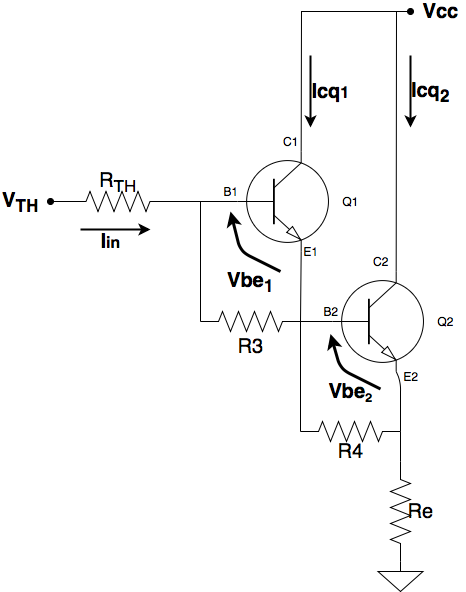
\includegraphics[scale=0.4]{./Imagenes/polarizacion.png} \\
			\caption{Circuito equivalente para el an\'alisis de polarizaci\'on.}
			\label{polarizacion}
		\end{figure}

Los valores utilizados para los cálculos son los de los componentes que utilizados en la implementación del circuito, que fueron elegidos en base a las simulaciones realizadas, con el fin de lograr un resultado óptimo. De esta forma, los valores de los componentes utilizados se listan en la Tabla \ref{tabla_valores}. Los transistores utilizados son BC337-40.

\begin{table}[H]
\centering
\begin{tabular}{ll}
\hline
\multicolumn{2}{l}{\begin{tabular}[c]{@{}l@{}}Parámetros\\   del circuito\end{tabular}} \\ \hline
$V_{cc}$                                     & 15,00E+00                                     \\
$R_1$                                         & 100,00E+03                                    \\
$R_2$                                         & 330,00E+03                                    \\
$R_s$                                         & 10,00E+03                                     \\
$R_3$                                         & 10,00E+03                                     \\
$R_E$                                         & 4,70E+03                                      \\
$R_L$                                         & 1,00E+03                                   
\end{tabular}
\caption{Valores de los componentes utilizados}
\label{tabla_valores}  
\end{table}

El equivalente de Thevenin entre la base del primer transistor y masa se obtiene mediante:\\

	\begin{equation}
		\begin{cases}
		&V_{TH} = \frac{R_2}{R_1 + R_2} V_{CC}\\ \\
		&R_{TH} = R_1 // R_2 
		\end{cases}
		\label{Thevenin}
	\end{equation}

Recorriendo la malla de entrada se tiene que:
\begin{equation}
		V_{th}-I_{B1}R_{th}-V_{BEon_{1}}-V_{BEon_{2}}-R_{e}(I_{E_{2}}+I_{R_{3}})=0 
\end{equation}
Del nodo que conecta el emisor del primer transistor con la base del segundo, se relacionan las corrientes de los transistores:
\begin{equation}
		I_{B_{2}} = I_{E_{1}} - \frac{V_{BEon_{2}}}{R_{3}}
\end{equation}
Por último, de las ecuaciones de cada transistor, despreciando el efecto de las $I_{CB0}$ dado que se trabaja a temperatura ambiente, se verifica:

	\begin{equation}
		\begin{cases}
		Q_{1}) \, \, I_{E_{1}} = I_{B_{1}}(\beta_{1}+1)\\ \\
		Q_{2}) I_{E_{2}}=I_{B_{2}}(\beta_{2}+1)
		\end{cases}
	\end{equation}

Resolviendo dichas ecuaciones se llega a las siguientes expresiones para las corrientes de colector de ambos transistores:

	\begin{equation}
		\begin{cases}
		I_{cq_{1}}=\frac{V_{th}-V_{BEon_{1}}-V_{BEon_{2}}\left(1-\frac{R_{e}\beta_{2}}{R_{3}}\right)}{\frac{R_{th}}{\beta_{1}}+R_{e}\beta_{2}}\\ \\
		I_{cq_{2}}=V_{th}\frac{1}{\frac{R_{th}}{\beta_{1}\beta_{2}}+R_{e}\frac{\beta_{2}+1}{\beta_{2}}}-V_{BEon_{1}}\frac{1}{\frac{R_{th}}{\beta_{2}}+R_{e}\beta_{1}}-V_{BEon_{2}}\left(\frac{\beta_{2}}{R_{3}}+\frac{\left(1-\frac{R_{e}\beta_{2}}{R_{3}}\right)\cdot(\beta_{1}+1)}{\frac{R_{th}}{\beta_{2}}+R_{e}\beta_{1}} \right)
		\end{cases}
	\end{equation}

Por último, se puede verificar que ambos transistores queden correctamente polarizados mediante:

	\begin{equation}
		\begin{cases}
		V_{CEQ_{1}}=V_{CC}-V_{BEon_{2}}\left(1+\frac{R_{e}}{R_{3}}\right)-R_{e}I_{CQ_{2}}\\ \\
		V_{CEQ_{2}}=V_{CC}-V_{BEon_{2}}\frac{R_{e}}{R_{3}}-R_{e}I_{CQ_{2}}
		\end{cases}
	\end{equation}
	

Para los cálculos se utiliza $V_{BEon}=0.7(V)$ para ambos transistores. Con respecto a los $H_{FE}$, éstos dependen de las $I_{CQ}$ según la \href{https://pdf1.alldatasheet.com/datasheet-pdf/view/171970/ONSEMI/BC337-40.html}{hoja de datos del fabricante}, con lo que son distintos para cada transistor. Tomando inicialmente el $H_{FE}$ mínimo de la hoja de datos, e iterando para los valores de $I_{CQ}$ obtenidos, se llega a que:
	\begin{equation*}
		\begin{cases}
		 H_{FE1} = 47\\
		 H_{FE2} = 90
		\end{cases}
	\end{equation*}
Reemplazando además por los valores de los componentes utilizados, se hallan los valores de $I_{cq_{1}}$, $I_{cq_{2}}$, $V_{CEQ_{1}}$ y $V_{CEQ_{2}}$, detallados en la Tabla \ref{tabla_valores_polarizacion}.

\begin{table}[H]
	\centering
\begin{tabular}{ll}
\multicolumn{2}{l}{Polarización} \\ \hline
ICQ1          & 93,54E-06        \\
ICQ2         & 2,12E-03         \\
VCEQ1         & 4,01E+00         \\
VCEQ2         & 4,71E+00        
\end{tabular}
\caption{Valores hallados para las componentes de polarizacion.}
\label{tabla_valores_polarizacion}  
\end{table}


	\subsection{Modelo incremental}
	
	Los estimadores para los parámetros del modelo incremental de cada transistor se detallan a continuación.

		\begin{equation}
			\begin{cases}
			\widehat{r_{e}}=\frac{V_{T}}{I_{CQ}}\\
			\widehat{h_{ie}}=(\beta+1)R_{e}\\	
			\widehat{gm}=\frac{1}{r_{e}}\\
			\widehat{hfe}= \beta_{DC}\\
			\widehat{1/hoe}= \infty
			\end{cases}
			\label{mod_inc_ecs}
		\end{equation}
		
	Se utiliza la ganancia de continua como estimador dado que las hojas de datos no especifican un valor para $h_{fe}$. Utilizando los valores de las corrientes de polarización y $h_{fe}$ de cada transistor, se obtienen los siguientes valores:
	
	\todo{COMPLETAR TABLA de estimadores}
	\begin{table}[h!]
		\centering
		\begin{tabular}{c c c}%
			\bfseries Estimadores & Q1 & Q2 \\ \hline
			$\widehat{g}_m$ &  & \\
			$\widehat{h}_{ie}$ &  & \\
			$\widehat{r}_{e}$&  & \\
			\hline
		\end{tabular}
		\caption{Estimadores correspondientes al modelo incremental, para los transistores Q1 y Q2.}
		\label{avolf}
	\end{table}
	
	\subsection{Circuito incremental}
	
	En la Figura \ref{circ_incremental} se muestra el circuito incremental. Las resistencias de salida de cada transistor se desprecian en los cálculos ya que hacerlo no introduce un error considerable y simplifica las operaciones.
		\begin{figure}[H]
			\centering
			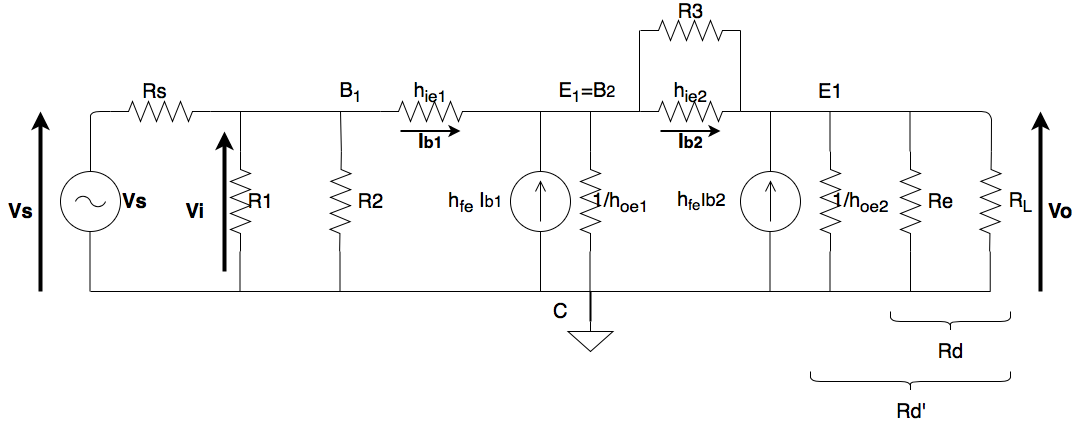
\includegraphics[scale=0.4]{./Imagenes/circ_incremental.png} \\
			\caption{Circuito equivalente para el an\'alisis del circuito incremental.}
			\label{circ_incremental}
		\end{figure}

En la Tabla \ref{tabla_valores_incremental} se muestran los valores utilizados y calculados en esta sección, que se utilizan para calcular las ganancias e impedancias del circuito.

\begin{table}[H]
\centering
\begin{tabular}{ll}
\multicolumn{2}{l}{Modelo incremental} \\ \hline
VT              & 26mV             \\
hfe1            & 47            \\
hfe2            & 90            \\
hie1            & 13,34$k\Omega$            \\
hie2            & 1,12$k\Omega$             \\
\end{tabular}
\label{tabla_valores_incremental} 
\end{table}

Para poder resolver el circuito fácilmente, se agrupa en paralelo la resistencia $R_3$ con $hie2$. Para poder hacerlo, se debe también adaptar la fuente de corriente del segundo transistor por la que circula por el paralelo de las resistencias de la siguiente forma. Además, se agrupan en paralelo $R_e$ y $R_L$. Para éstas consideraciones se calculan los siguientes parámetros:

	\begin{equation}
		\begin{cases}
		hfe_{2}^{*}=hfe_{2}\frac{R_{3}}{R_{3}+hie_{2}} \\
		hie_{2}^{*}=hie_{2}//R_{3} \\
		R_{d}=R_{e}//R_{2}
		\end{cases}
		\label{mod_inc_ecs}
	\end{equation}

Reemplazando por los valores correspondientes se obtienen los siguientes valores:

\begin{table}[H]
\centering
\begin{tabular}{ll}
\multicolumn{2}{l}{Simplificaciones} \\ \hline
hfe2*          & 80,96           \\
Rd             & 824,56$\Omega$          \\
hie2*          & 1,00$k\Omega$          
\end{tabular}
\end{table}

A partir del circuito y de los cálculos anteriores, se puede ver que las expresiones para las impedancias que se ven a la entrada del primer transistor, del amplificador y del sistema se ven representadas por las ecuaciones que se muestran a continuación, utilizando pasaje a nivel de corriente. 

	\begin{equation}
		\begin{cases}	
		R_{i}=hie_{1}+(hfe_{1}+1)hie_{2}^{*}+(hfe_{2}^{*}+1)(hfe_{1}+1)R_{d} \\
		R_{ia}=R_{i} // R_{th} \\
		R_{is}=R_{s}+R_{ia}
		\end{cases}
		\label{mod_inc_ecs}
	\end{equation}

De donde reemplanzando por los valores ya calculados se obtienen las impedancias de entrada:

\begin{table}[H]
\centering
\begin{tabular}{ll}
\multicolumn{2}{l}{\begin{tabular}[c]{@{}l@{}}Impedancias\\   de entrada\end{tabular}} \\ \hline
Ri                                      & 3,31$M\Omega$                                     \\
Ria                                     & 75,00$k\Omega$                                    \\
Ris                                     & 85,00$k\Omega$                                   
\end{tabular}
\end{table}

Para el cálculo de la ganancia de tensión del sistema primero se calcula:

	\begin{equation}
		\begin{cases}	
		\frac{V_{o}}{ib_{2}^{*}}=R_{d}(hfe_{2}^{*}+1) \\
		\frac{V_{i}}{V_{s}}=\frac{R_{ia}}{R_{ia}+R_{s}}
		\end{cases}
		\label{mod_inc_ecs}
	\end{equation}

Así la ecuación de la ganancia en tensión del sistema se puede expresar de la siguiente forma. \\

	\begin{equation}	
		\Delta _{vs}=\frac{V_{o}}{V_{s}}=\frac{V_{o}}{ib_{2}^{*}}\cdot\frac{ib_{2}^{*}}{ib_{1}}\cdot\frac{ib_{1}}{V_{i}}\cdot\frac{V_{i}}{V_{s}}=R_{d}(hfe_{2}^{*}+1)(hfe_{1}+1)\frac{1}{R_{i}}\frac{Ria}{Ria+Rs}
		\label{mod_inc_avs}
	\end{equation}

Finalmente, se llega a los valores de las ganancias de tensión del amplificador y del sistema:

\begin{table}[H]
\centering
\begin{tabular}{ll}
\multicolumn{2}{l}{\begin{tabular}[c]{@{}l@{}}Ganancias\\   de tension\end{tabular}} \\ \hline
Av                                       & 0,981                                     \\
Avs                                      & 0,866                                    
\end{tabular}
\end{table}

Al ser la configuración colector común se esperaba una ganancia de tensión menor a 1. De éste resultado se puede observar una ventaja de la configuración Darlington con respecto al colector común con un solo transistor, ya que éste último no puede llegar valores de ganancia de tensión superiores al 80\%.\\
Para el cálculo de la ganancia de corriente se utiliza:

	\begin{align*}
		\Delta _{i} &= \frac{I_{Rd}}{ib_{1}}=(hfe_{2}^{*}+1)(hfe_{1}+1) \\
%
	\Delta_{is} &= \frac{I_{Rd}}{I_{Rs}}\cdot\frac{I_{b_{1}}}{I_{Rs}}=\frac{R_{th}}{R_{th}+R_{i}}\Delta_{i} \\
%
		\Delta_{is}^{\, \, \,'} &= \frac{I_{Rl}}{I_{Rs}}=\frac{I_{Rl}}{I_{Rd}}\cdot\frac{I_{Rd}}{I_{Rs}}=\frac{R_{e}}{R_{e}	+R_{2}}\Delta_{is}
%
		\label{mod_inc_ais}
	\end{align*}


Donde $\Delta_{i}$ es la ganancia de corriente, $\Delta_{is}$ es la ganancia de corriente del sistema y $\Delta_{is}^{\, \, \,'}$ es la ganancia de corriente del sistema sobre la carga. En $\Delta_{i}$ se puede apreciar la gran ganancia de corriente que tiene esta configuración, ya que se multiplican las ganancias de cada transistor. Los valores de las mismas se muestran en la siguiente tabla:

\begin{table}[H]
\centering
\begin{tabular}{ll}
\multicolumn{2}{l}{\begin{tabular}[c]{@{}l@{}}Ganancias\\   de corriente\end{tabular}} \\ \hline
Ai                                       & 3934,08                                     \\
Ais                                      & 89,27                                       \\
Ais'                                     & 73,61                                      
\end{tabular}
\end{table}

Para la resistencia de salida, se pasiva la entrada, se coloca a la salida una fuente $V_{op}$ con el terminal positivo a masa, y se calcula la corriente $I_{op}$ que circula por dicha fuente. Las siguientes relaciones se utilizan para el cálculo:

	\begin{equation}
		\begin{cases}	
		V_{op}=I_{B1}( R_{s}//R_{th}+h_{ie1} + hfe_{1}+1)hie_{2}^{*}) \\
		I_{op}=I_{B1}(hfe_{1}+1)(hfe_{2}^{*}+1)\\
		r_{o}=\frac{V_{op}}{I_{op}}=\frac{R_{s}//R_{th}+hie1+(hfe1+1)hie_{2}^{*}}{(hfe_{1}+1)(hfe_{2}^{*}+1)}\\
		r_{oa}=R_{e}//r_{o}\\
		r_{os}=r_{oa}//R_{L}
		\end{cases}
		\label{mod_inc_ro}
	\end{equation}

Reemplazando por los valores de las variables involucradas en la ecuación, se obtienen los valores de las resistencias de salida vistas a la salida del segundo transistor, a la salida del amplificador y luego de la carga.

\begin{table}[H]
\centering
\begin{tabular}{ll}
\multicolumn{2}{l}{Impedancias de salida} \\ \hline
ro                & 15346,62              \\
roa               & 3598,07               \\
ros               & 782,52               
\end{tabular}
\end{table}
